\documentclass[conference]{IEEEtran}
\IEEEoverridecommandlockouts
\usepackage{cite}
\usepackage{amsmath,amssymb,amsfonts}
\usepackage{algorithmic}
\usepackage{graphicx}
\usepackage{textcomp}
\usepackage{xcolor}
\usepackage{float}
\usepackage{graphicx}
\usepackage{float}


\floatstyle{boxed} 
\restylefloat{figure}

\def\BibTeX{{\rm B\kern-.05em{\sc i\kern-.025em b}\kern-.08em
    T\kern-.1667em\lower.7ex\hbox{E}\kern-.125emX}}
\begin{document}

\title{Report: Sleep State Prediction Using Accelerometry Data}

\author{
	\IEEEauthorblockN{Juan Carlos Quintero Rubiano}
	\IEEEauthorblockA{Code: 20232020172\\
		\textit{Systems Engineering} \\
		\textit{Francisco Jose de Caldas District University}\\
		Bogota, Colombia \\
		jcquineror@udistrital.edu.co}\\
	\IEEEauthorblockN{Juan Felipe Wilches Gomez}
	\IEEEauthorblockA{Code: 20231020137\\
		\textit{Systems Engineering} \\
		\textit{Francisco Jose de Caldas District University}\\
		Bogota, Colombia \\
		jfwilchesg@udistrital.edu.co}
	\and
	\IEEEauthorblockN{Juan Nicolas Diaz Salamanca}
	\IEEEauthorblockA{Code: 20232020059\\
		\textit{Systems Engineering} \\
		\textit{Francisco Jose de Caldas District University}\\
		Bogota, Colombia \\
		jndiazs@udistrital.edu.co}
}

\maketitle

\begin{abstract}
	El sueño es fundamental en el correcto funcionamiento de diferentes sistemas internos de nuestro cuerpo, siendo el mas importante el sistema de limpieza del cerebro el cual es mas eficiente cuando se duerme, es por esta razon que se estudia la calidad del sueño clasificandolo en estados, el sueño no REM dividido en 3 partes, y el sueño REM en el cual el sistema de limpieza del cerebro es mas eficaz
    
    The study of sleep is crucial for diagnosing sleep disorders; however, the traditional method, polysomnography (PSG), is costly and impractical for long-term use. This paper presents a systematic computational approach to predict sleep states using accelerometry data from low-cost, non-invasive wrist-worn devices. Movement patterns (ENMO, Anglez) are analyzed through a five-stage pipeline: acquisition, preprocessing, feature extraction, classification, and validation.
\end{abstract}

\section{Introduction}

\section{Objectives}

\section{State Of The Art}

La polisomnografia es el estandar de referencia para la evaluacion del sueño, ya que permite la clasisificacion detallada de los estados de sueño mediante registros fisiologicos como EEG, EOG y EMG, sin embargo esta tecnica esta limitada por ser invasiva, costosa y compleja requiriendo personal medico especializado y un entorno controlado.

Es por esto que han surgido metodos alternativos basados en la acelerometria, que utilizan sensores de movimiento incorporados en dispositivos como manillas o relojes inteligentes, estos permiten detectar estados de sueño y vigilia a travez de patrones de movimiento, dando la posibilidad a que sea mas accesible gracias a su bajo costo y eficiente a largo plazo. Diferentes estudios han evidenciado que aunque estos metodos no alcanzan la presicion de la polisomnografia para distingir entre las etapas del sueño no REM (N1, N2, N3), si son efectivos y confiables para la clasificacion binaria entre sueño y vigilia.

Se presenta un enfoque sistematico y computacional para la prediccion de estados de sueño mediante datos recolectados de acelerometria. El pipeline se compone de la adquisicion de datos, preprocesamiento, la extraccion de caracteristicas, la clasificación y finalmente la prediccion de estados futuros. Todo este proceso se apoya en modelos computacionales como algoritmos basados en umbrales como Sadeh y Cole-Kripke y redes neuronales profundas, incluyendo LSTM, que capturan dependencias temporales en los datos.


\section{Mathematical model:}

		In order to simulate sleep and awake dynamics, we determine the probability of movement, sleep and the dynamic transition between 
		involuntary and voluntary movements. The model is based on a logistic regression that describes the differents variables involved 
		it and its weight on the probability to be converted into a probability value, range on 0 and 1 via sigmoid function:
		
    \begin{equation}
       ln(\frac{p}{1-p}) = \beta_0 + \beta_1x_1 + \beta_2x_2 ...+\beta_nx_n 
		\end{equation}
	\center
	Logistic regression equation
    
		\begin{equation}
			\sigma =\frac{1}{1-e^{-x}}
		\end{equation}
	\center 
	Sigmoid function
	\\
  \raggedright
	We applied both equation to generate the probability as following equation:

		\[ p = \frac{1}{1-e^{(\beta_0 + \beta_1x_1 + \beta_2x_2 ...+\beta_nx_n)}} \]	

\section{Simulation Development}

Based on the logistic regression model we create the simulation following the next steps

\subsection{Planning}

In order to apply the mathematical model, we need to define the variables and their respective weights.
The variables are based on the entries of the simulation, and the weights are determined by the 
importance of each variable in the probability of movement, sleep, and transition between involuntary
and voluntary movements.

\subsubsection{Entries}
\begin{itemize}
	\item \textbf{Light (lux)}: Simulate light ambiental intesity variability between day and night.
	\item \textbf{Sound (dB)}: Simulate sound level variability between a noisy and silent environment.
	\item \textbf{Stress}: Simulate a ssubjective scale of psychological and physical stress.
	\item \textbf{physical activity (proxy ENMO)}: A static or simulate physical activity level, if it is
	simulate, it will base on movement probability.
	\item \textbf{ENMO (g)}: Entries simulate via a normal distribution consequence of a involuntary
	movement, determined by movement probability.
	\item \textbf{Anglez (°)}: Entries simulate via a normal distribution consequence of a
	voluntary movement, determined by movement probability.
\end{itemize}

\subsubsection{Probability functions}
\begin{itemize}
	\item \textbf{Movement probability}: The probability of movement is determined by the light, sound, stress and physical activity variables.
	\\
	\[ P_{move} = \sigma(\beta_0 + \beta_{lux}*x_{lux} + \beta_{dB}*x_{dB} \]
	\[+ \beta_{stress}*x_{stress} + \beta_{sleep} * \cdot I_{sleep}) \]
	\\
	Where $I_{sleep}$ is an indicator variable that is 1 if the subject is sleeping and 0 otherwise.
	\\
	\item \textbf{Sleep probability}: The probability of sleep is determined by the light, sound, stress and physical activity variables.
	
	\[ P_{sleep} = \sigma(\alpha_0 + \alpha_{proxy ENMO}*x_{proxy ENMO}+ \alpha_{lux}*x_{lux}\]
	\[ + \alpha_{dB}*x_{dB} + \alpha_{stress}* x_{stress}) \]

\end{itemize}

\subsubsection{Simulation cycle}
The simulation cycle is based on the following steps:
\begin{enumerate}
	\item Light, Sound, Stress are uploaded based on a Gaussian noise.
	\item Every 12 steps, light and sound are updated randomly.
	\item probability of movement is calculated
	\item Movement is determined by stocastic process, if the movement
	probability is greater than a random number between 0 and 1, then
	the movement is determined
	\item if the movement is determined, then the ENMO and Anglez are calculated 
	with more variability, otherwise, they are calculated with less variability.
	\item Sleep probability is calculated 
	\item Graphic interface is updated with the new values of light, sound, stress, ENMO and Anglez.
\end{enumerate}

\subsubsection{Limitations}
The simulation is based on a simplified model of sleep which does not consider important
physiological data as EEG, EMG, EOG, and other variables that can affect the sleep state 
recollected via polysomnography. Also, the simulation consider the differents entries as 
independent variables, which is not the case in real life, where the variables can be correlated,
for example, the light and sound can be correlated, and the stress can be correlated 
with the physical activity. And chaos actions as micro-awakening, sleep apnea, and other
phenomena are not considered in the simulation, which can slant the entries variables 
and results or involuntary and voluntary movements can be difficult to determine in real life.

\subsection{Implementation}

The simulation is implemented in a JAVA application based on a MVC architecture,
using the JavaFX library for the graphical interface as view, module called 
simulation as model to calculate probability and set weights and controller
to connect simulation module with graphical interface.

\begin{figure}[H]
	\centering
	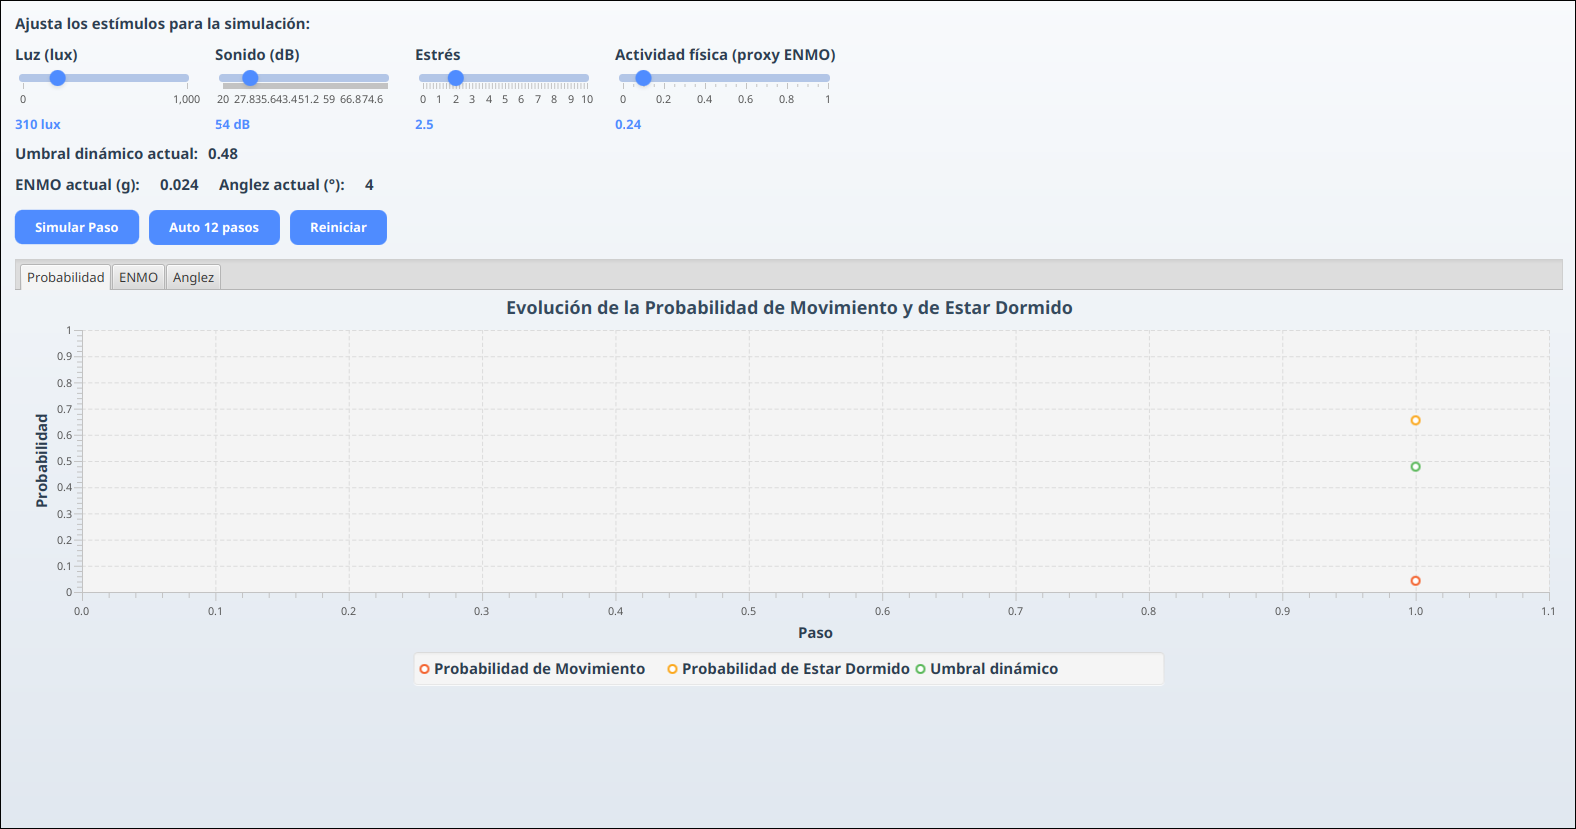
\includegraphics[width=\linewidth]{images/simulation_1.png}
	\caption{Simulation graphical interface with initial values}
\end{figure}

\begin{figure}[H]
	\centering
	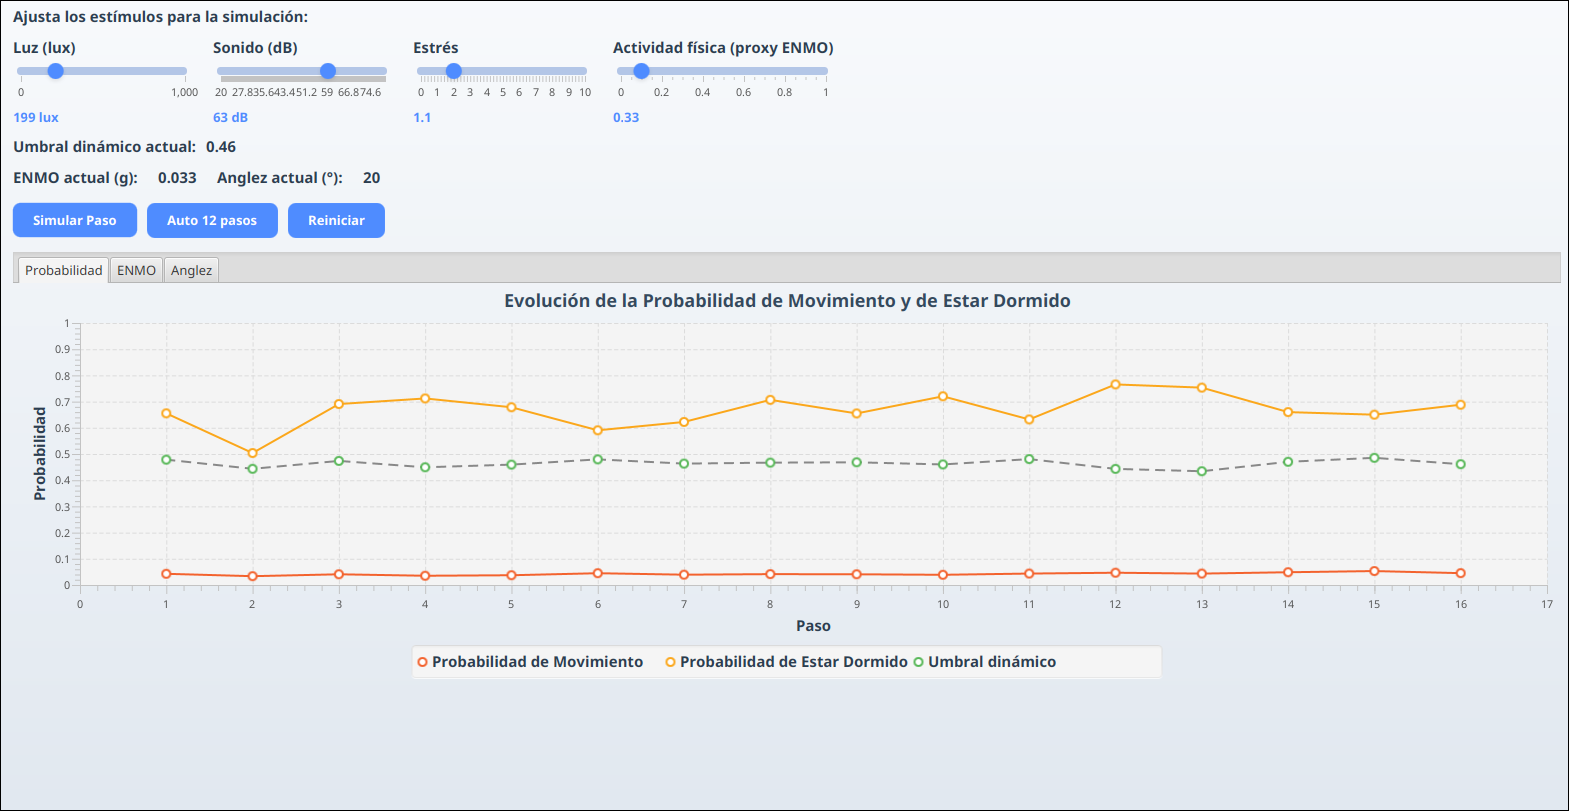
\includegraphics[width=\linewidth]{images/simulation_2.png}
	\caption{Simulation graphical interface with simulation steps}
\end{figure}
\subsection{Results}

\subsubsection{Chaos and sensitivity}

\begin{itemize}
	\item Gaussian noise is used to simulate the light, sound, activity and
	 stress variables, which introduce randomness in the probability predicted
	 making it more realistic.
  \item Every 12 steps light and sound change randomness simulated
  a change in the environment as turning light or open a window.
  \item Movement is decided in a stocastic way using the probability calculated
  and uniform random number generated.
	\item ENMO is generated by normal distribution of N(0.13, 0.04)
	altered by a range [0.05, 0.25] when a voluntary movement is determined and
	a normal distribution of N(0.025, 0.01) altered by a range[0.01, 0.05]
	\item Anglez is generated by voluntary and involuntary events, changing
  the range which angles varies, making anglez randomness consequence
	of the stocastic desicion of movement
	 
\end{itemize}

Through these conditions of chaos and sensitivity, environmental variables
as light and sound make the sleep probability chaotic and difficult to determine
in a long term however variables with less chaos as physical activity and 
stress are less variability and keep constant the movement probability however
due to stocastic process ENMO is chaotic and difficult to predicted

\begin{figure}[H]
	\centering
	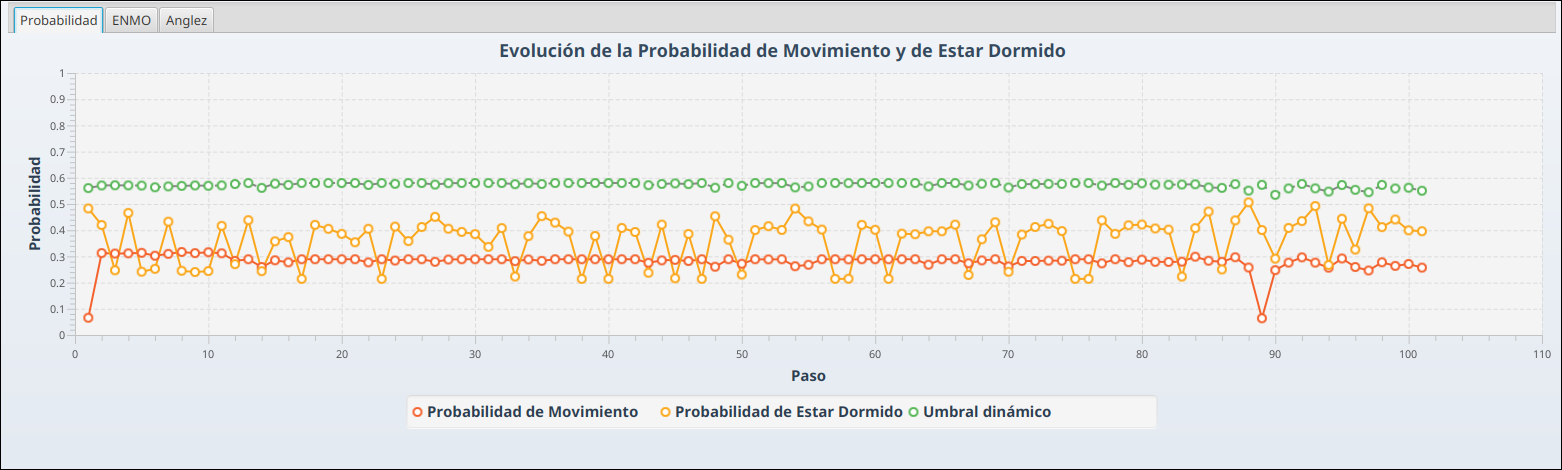
\includegraphics[width=\linewidth]{images/simulation_3.png}
	\caption{Simulation with highest stress level}
\end{figure}

\begin{figure}[H]
	\centering
	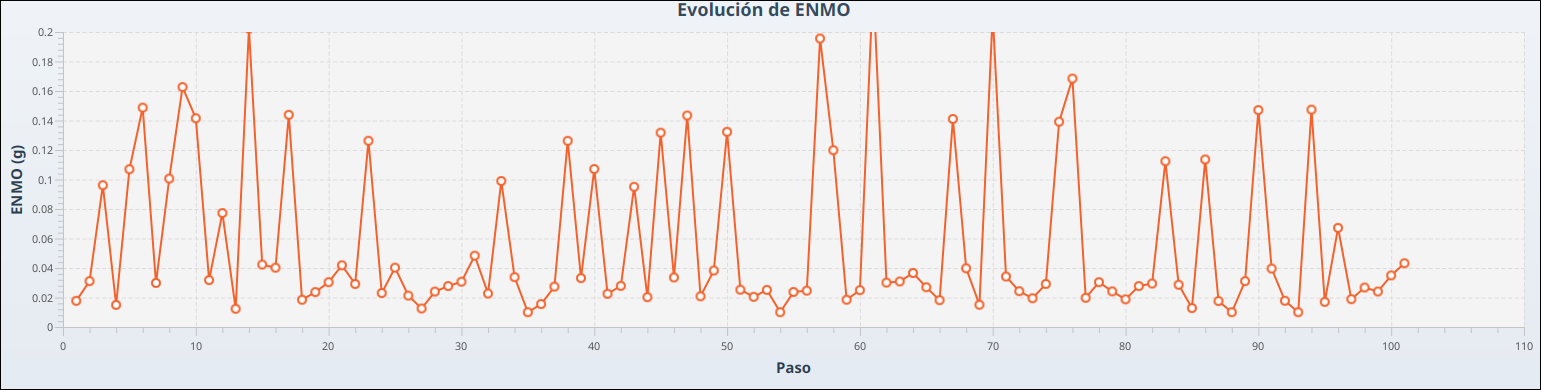
\includegraphics[width=\linewidth]{images/simulation_4.png}
	\caption{ENMO evolution with highest stress level}
\end{figure}

\begin{figure}[H]
	\centering
	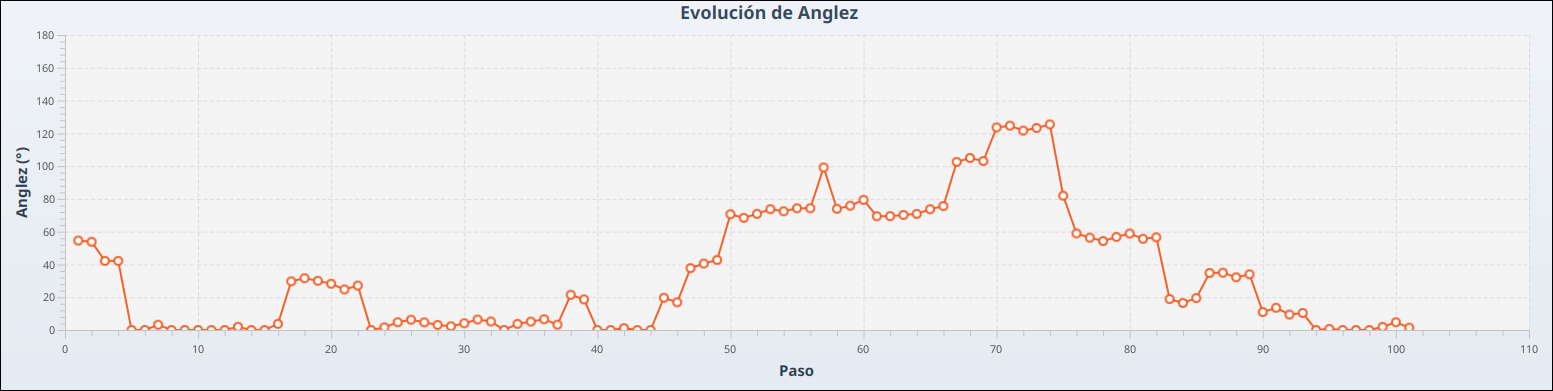
\includegraphics[width=\linewidth]{images/simulation_5.png}
	\caption{Anglez evolution with highest stress level}
\end{figure}

\begin{figure}[H]
	\centering
	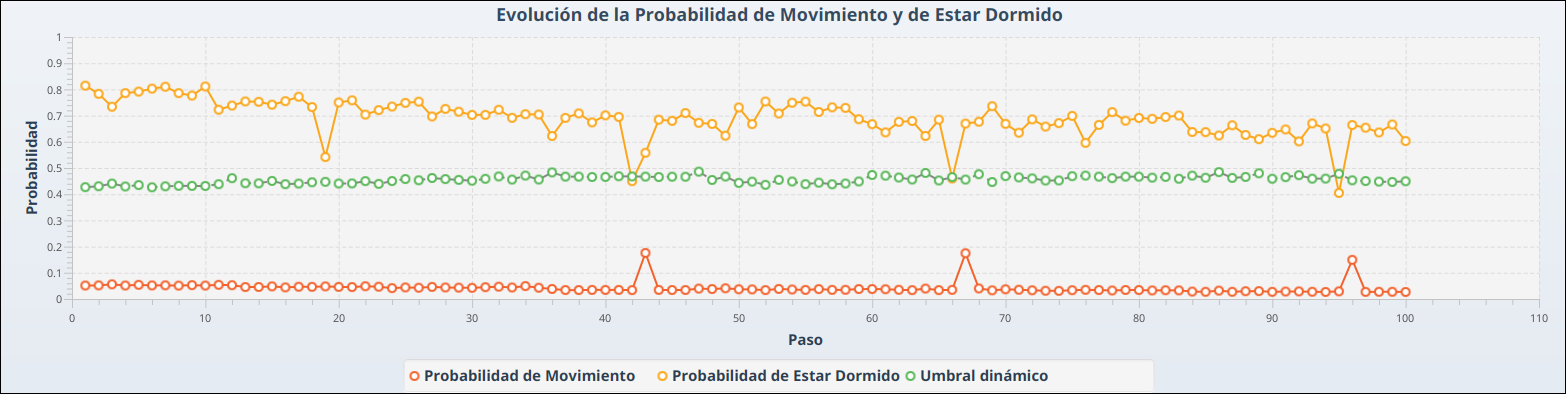
\includegraphics[width=\linewidth]{images/simulation_6.png}
	\caption{Simulation with lowest stress level}
\end{figure}

\begin{figure}[H]
	\centering
	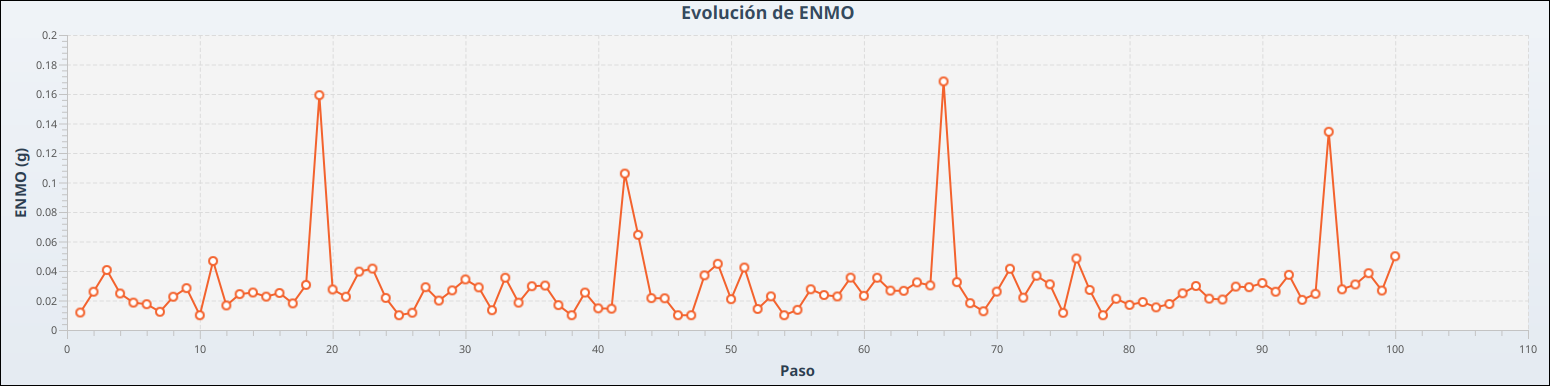
\includegraphics[width=\linewidth]{images/simulation_7.png}
	\caption{ENMO evolution with lowest stress level}
\end{figure}

\begin{figure}[H]
	\centering
	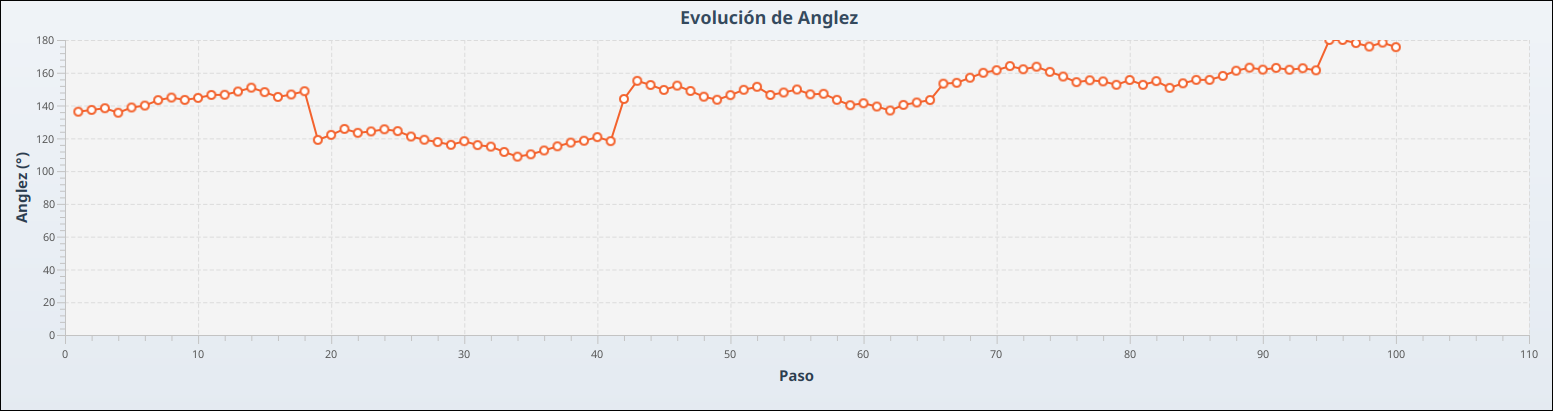
\includegraphics[width=\linewidth]{images/simulation_8.png}
	\caption{Anglez evolution with lowest stress level}
\end{figure}

However a less stress level generate a simulation less sensitive to the 
chaos from light and sound, as a consequence an ENMO and Anglez are constant
in a long term. Based on the simulation result we can conclude stress level 
are fundamental to keep sleep state in a long term than light and sound. 



\end{document}